\documentclass[border=8pt, multi, tikz]{standalone}
\usepackage{import}
\usepackage{graphicx}
\usetikzlibrary{shapes, arrows, 3d}
\subimport{../layers/}{init}
\def\input_image{../examples/input.jpg}
\def\skyseg{../examples/sky_segmentation.png}
\def\cloudseg{../examples/cloud_seg.png}

\begin{document}
	\begin{tikzpicture}
	\tikzstyle{fillwhite} = [fill=white,inner sep=0pt, opacity=1]
	\tikzstyle{connection}=[ultra thick,every node/.style={sloped,allow upside down},draw=\edgecolor,opacity=0.7]
	
% Real Image

	\pic[shift={(0, 0, 0)}] at (0,0,0)	
	{SolidBox={
		name=input_image,
		caption=\huge \bf Input image,
		fill=gray,
		height=20,
		depth=20,
		width={1}
		}
	};

	\pic[shift={(4, 0, 0)}] at (input_image-east)	
	{SolidBox={	
			name=backbone,
			label=\huge \bf Backbone,
			fill=gray,
			height=8,
			depth=8,
			opacity=0.1,
			width={25}
		}
	};

	\draw [connection] (input_image-east) -- node [coordinate] (test) {} (backbone-west);
	\path (test) -- node [fillwhite] {\midarrow} (backbone-west); 
	
	\pic[shift={(8, 0, 12)}] at (backbone-east)
	{SolidBox={
			name=attributes,
			label=\huge \bf Attribute \\ \huge \bf Estimation,
			fill=gray,
			height=8,
			depth=8,
			width={25}
		}
	};
%	\path (backbone-south) |- node [coordinate] (dummy_0) {} (attributes-west);
%	\draw [connection] (backbone-south) -- (dummy_0) -- node [fillwhite] {\midarrow} (attributes-west);

%	\draw [connection] (dummy_0) ++(0,-1) -| node [fillwhite, near start, rotate=180] {\midarrow} (attributes-nearsouth);

	\pic[shift={(10, 0, 0)}] at (backbone-east)
	{SolidBox={
			name=sky,
			label=\huge  \bf Sky \\ \huge  \bf Segmentation,
			fill=gray,
			height=8,
			depth=8,
			width={25}
		}
	};
	
	\pic[shift={(12, 0, -12)}] at (backbone-east)
	{SolidBox={
			name=cloud,
			label=\huge \bf Cloud \\ \huge \bf Segmentation,
			fill=gray,
			height=8,
			depth=8,
			width={25}
		}
	};	

	\pic[shift={(4, 0, 0)}] at (sky-east)	
	{SolidBox={
			name=output_seg,
			fill=white,
			height=20,
			depth=20,
			width={0.5}
		}
	};

	\pic[shift={(4, 0, 0)}] at (cloud-east)	
	{SolidBox={
			name=output_cloud_seg,
			fill=white,
			height=20,
			depth=20,
			width={0.1}
		}
	};

	\node[canvas is zy plane at x=0, shift=({0,0,0})] (image_1) at (input_image-east) {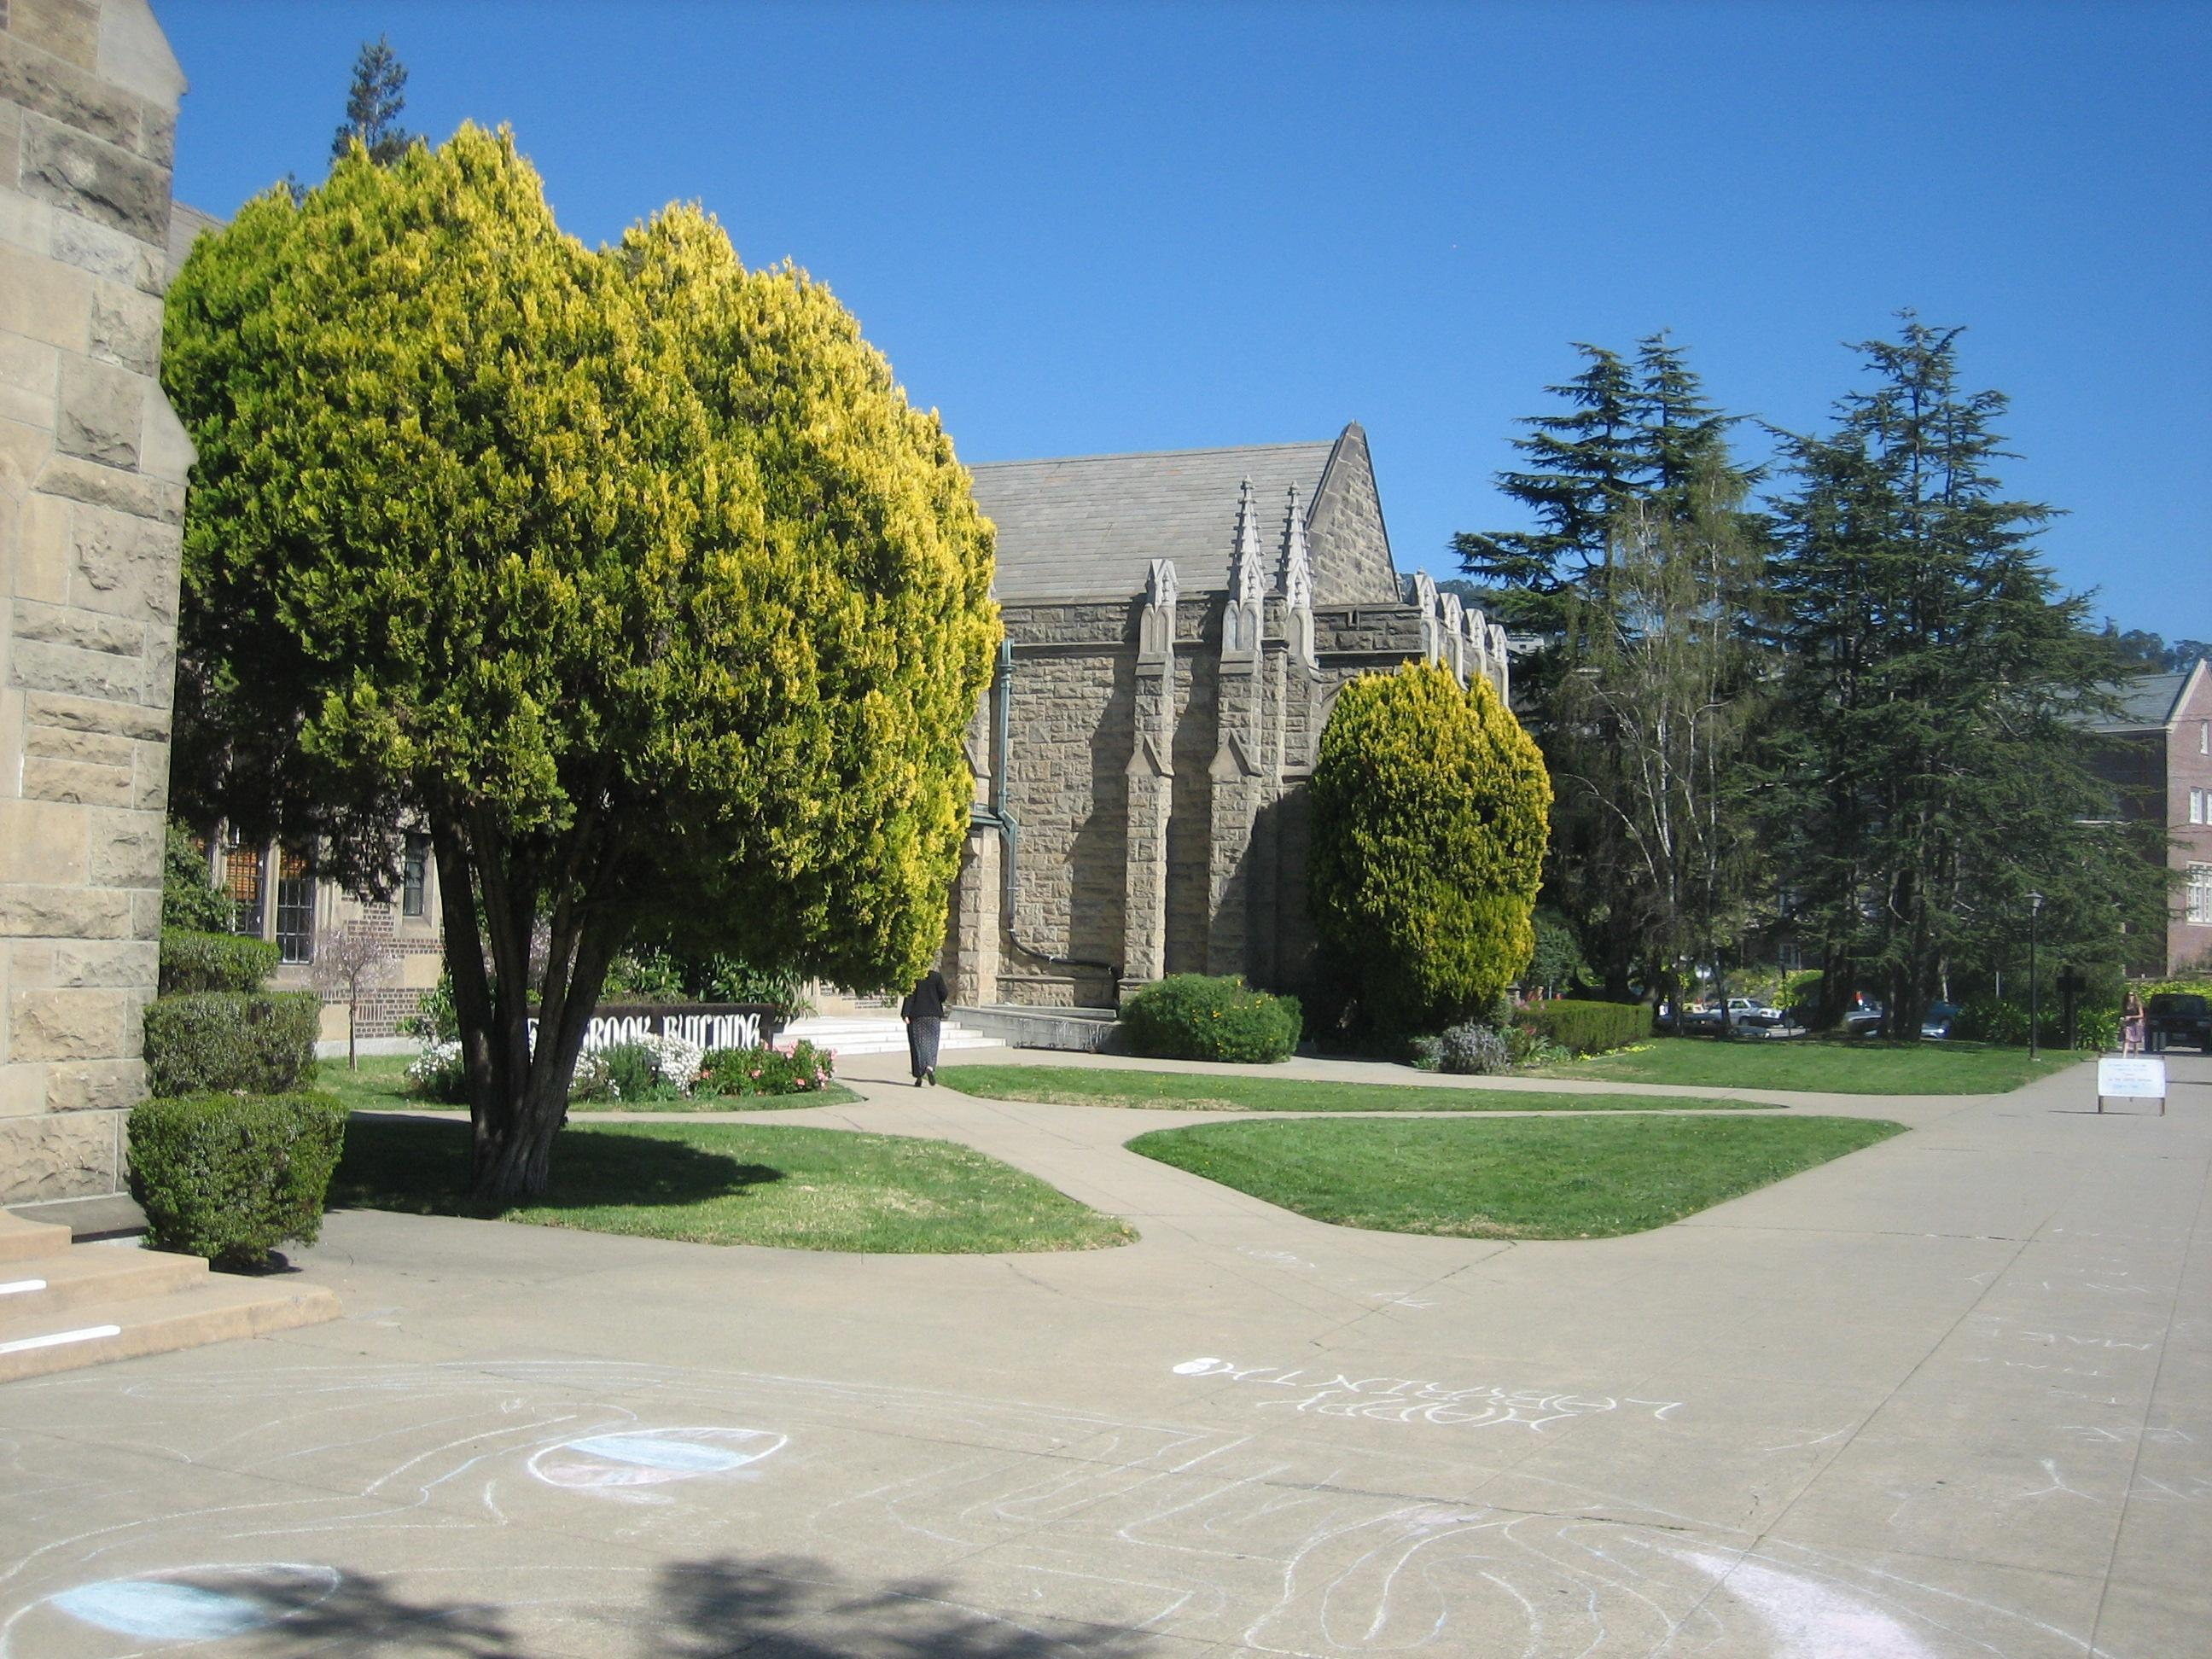
\includegraphics[width=4cm ,height=4cm ]{\input_image}};
	
	\node[canvas is zy plane at x=0, shift=({0,0,0})] (sky_seg) at (output_seg-east) {\includegraphics[width=4cm ,height=4cm ]{\skyseg}};
	
	\node[canvas is zy plane at x=0, shift=({0,0,0})] (cloud_seg) at (output_cloud_seg-east) {\includegraphics[width=4cm ,height=4cm ]{\cloudseg}};



	\path (backbone-east) -- node [coordinate, pos=0.3] (dummy_0) {} (sky-west);

	\draw [connection] (dummy_0) -- node [] {} ++(0,0,12) -| node [fillwhite, near start] {\midarrow} (attributes-west);	

	\draw [connection] (attributes-east) -| node [] {} ++(0.75,0,0) -- node {\midarrow} (sky-nearsouth);	
	\draw [connection] (backbone-east) -- node [fillwhite] {\midarrow} (sky-west);

	\draw [connection] (dummy_0) -- node [] {} ++(0,0,-12) -| node [fillwhite, near start] {\midarrow} (cloud-west);		
	\draw [connection] (sky-east) -| node [] {} ++(0.5,0,0) -- node {\midarrow} (cloud-nearsouth);	
	
	\node (att_results_1) [shift={(3,1,0)}, inner sep=15, anchor=west] at (attributes-east) {\LARGE \bf{Season [Spring, Summer, Autumn, Winter]}};
	\node (att_results_2) [shift={(3,0,0)}, inner sep=15, anchor=west] at (attributes-east) {\LARGE \bf{Time [Day, Night, Sunrise/Sunset, Dusk/Dawn]}};
	\node (att_results_3) [shift={(3,-1,0)}, inner sep=15, anchor=west] at (attributes-east) {\LARGE \bf{Weather [Sunny, Snow, Rain, Fog]}};
	\draw [connection] (attributes-east) -- node [pos=1] {\midarrow} (att_results_2.west);
	\node [draw,thick,minimum width=14.75cm,minimum height=3.5cm] (rect) at (att_results_2)  {};
	\draw [connection] (sky-east) -- node [pos=0.6] {\midarrow} (output_seg-west);	
	\draw [connection] (cloud-east) -- node [pos=0.6] {\midarrow} (output_cloud_seg-west);	
	

%	\pic[shift={(0, 0, 0)}] at (0,0,0)	
%	{SolidBox={
%			name=input_image,
%			caption=\LARGE \bf Input image,
%			fill=gray,
%			height=15,
%			depth=15,
%			width={1}
%		}
%	};

	


%	
%	\pic[shift={(2, 0, 0)}] at (real_images-east)
%	{SolidBox={
%			name=real_images_2,
%			fill=white,
%			height=15,
%			depth=15,
%			width={1, 1}
%		}
%	};
%	\path (real_images-east) -- node (real) {$\dots$} (real_images_2-west);
%	\node [shift={(1.25,0,0)}, below] at (real_images-nearsouth) {\LARGE \bf Real images};
%
%	\pic[shift={(4, 0, 0)}] at (generator-east)
%	{SolidBox={
%		name=fake_image,
%		fill=white,
%		height=15,
%		depth=15,
%		width={1}
%		}
%	};
%	\draw [connection] (generator-east) -- node [fillwhite] {\midarrow} (fake_image-west);
%
%	\path (generator-northwest) -- node[coordinate, near start] (generator_north_1) {} (generator-northeast);
%	\path (generator-northwest) -- node[coordinate, near end] (generator_north_2) {} (generator-northeast);
%	\path (generator-nearsouthwest) -- node[coordinate, near start] (generator_south_1) {} (generator-nearsoutheast);
%	\path (generator-nearsouthwest) -- node[coordinate, near end] (generator_south_2) {} (generator-nearsoutheast);		
%
%% Attributes
%\pic[shift={(2, 4.25, 0)}] at (real_image-north)
%{SolidBox={
%		name=attributes,
%		label= Attribute \\ prediction,
%		fill=yellow,
%		height=5,
%		depth=5,
%		width={12}
%	}
%};
%
%\path (real_image-north) |- node [coordinate] (dummy_0) {} (attributes-west);
%
%\draw [connection] (real_image-north) -- (dummy_0) -- node [fillwhite] {\midarrow} (attributes-west);
%\draw [connection] (dummy_0) ++(0,-1) -| node [fillwhite, near start, rotate=180] {\midarrow} (attributes-nearsouth);
%
%% Segmentation
%\pic[shift={(1, 6.75, 0)}] at (real_image-north)
%{SolidBox={
%		name=semantic_map,
%		label= Semantic \\ segmentation,
%		fill=orange,
%		opacity=0.25,			
%		height=5,
%		depth=5,
%		width={12}
%	}
%};
%\node[canvas is zy plane at x=1.5, shift=({0,0,0}), inner sep=0] (image_0) at (semantic_map-east) {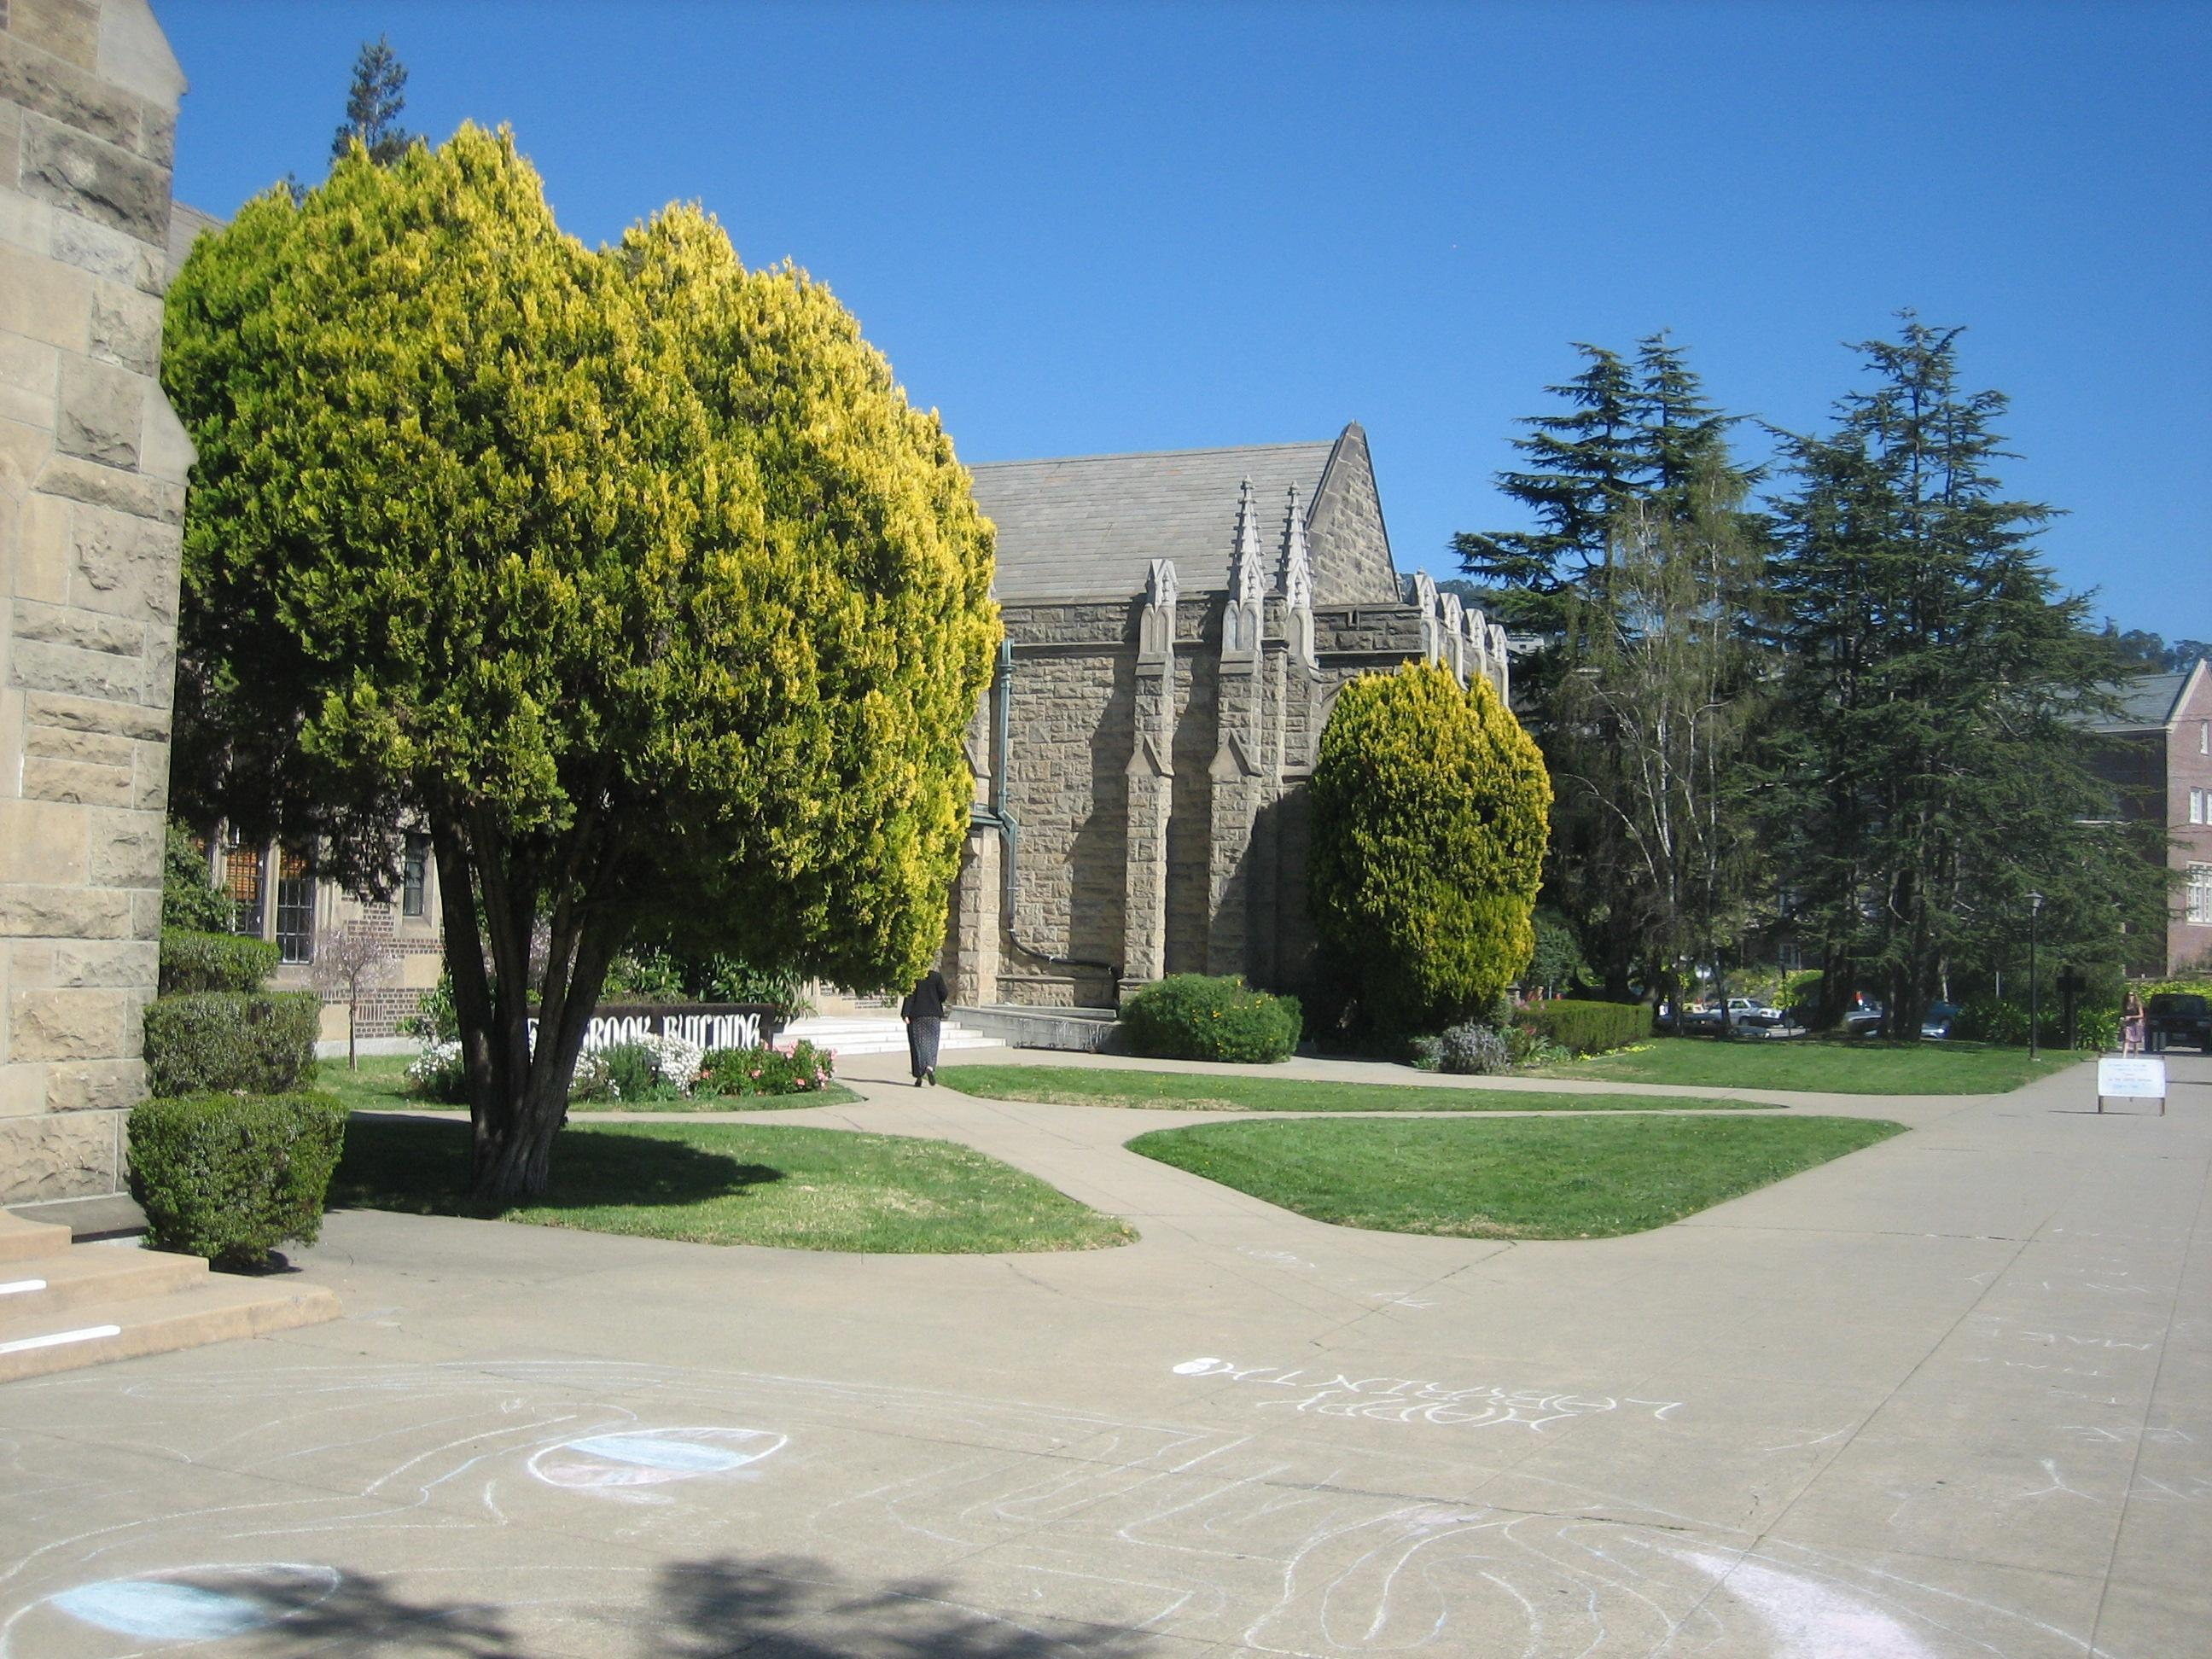
\includegraphics[width=2cm ,height=2cm ]{\input_image}};
%\draw [connection] (semantic_map-east) --(image_0);				
%\draw [connection] (dummy_0) |- node [pos=0.35, fillwhite] {\midarrow} (semantic_map-west);
%\draw [connection] (dummy_0) ++(0,1) -| node [fillwhite, near start, rotate=180] {\midarrow} (image_0.south);
%
%% Attribute Loss
%	\pic[shift={(-3.5, -3.5, 0)}] at (fake_image-south)
%	{SolidBox={
%			name=attributes_2,
%			label= Attribute \\ prediction,
%			fill=yellow,
%			height=5,
%			depth=5,
%			width={12}
%		}
%	};
%	\draw [connection] (fake_image-south) |- node [near start, fillwhite] {\midarrow} (attributes_2-east);	
%	\path (attributes_2-west) -| node[fillwhite, align=center] (att_loss) {\LARGE \bf\textit{Attribute}\\\LARGE \bf\textit{loss}} (generator_south_2);
%	\draw [connection] (attributes_2-west) -- node [fillwhite] {\midarrow} (att_loss);
%	\draw [connection] (random) |- node [near start, fillwhite] {\midarrow} (att_loss);
%	\draw [connection, densely dashed] (att_loss) -- node [fillwhite] {\midarrow}(generator_south_2);
%
%% Semantic Loss
%	\pic[shift={(-1, 6.75, 0)}] at (fake_image-north)
%	{SolidBox={
%			name=semantic_map_2,
%			label= Semantic \\ segmentation,
%			fill=orange,
%			opacity=0.25,	
%			height=5,
%			depth=5,
%			width={12}
%		}
%	};
%
%	\node[canvas is zy plane at x=-2, shift=({0,0,0})] (image_1) at (semantic_map_2-west) {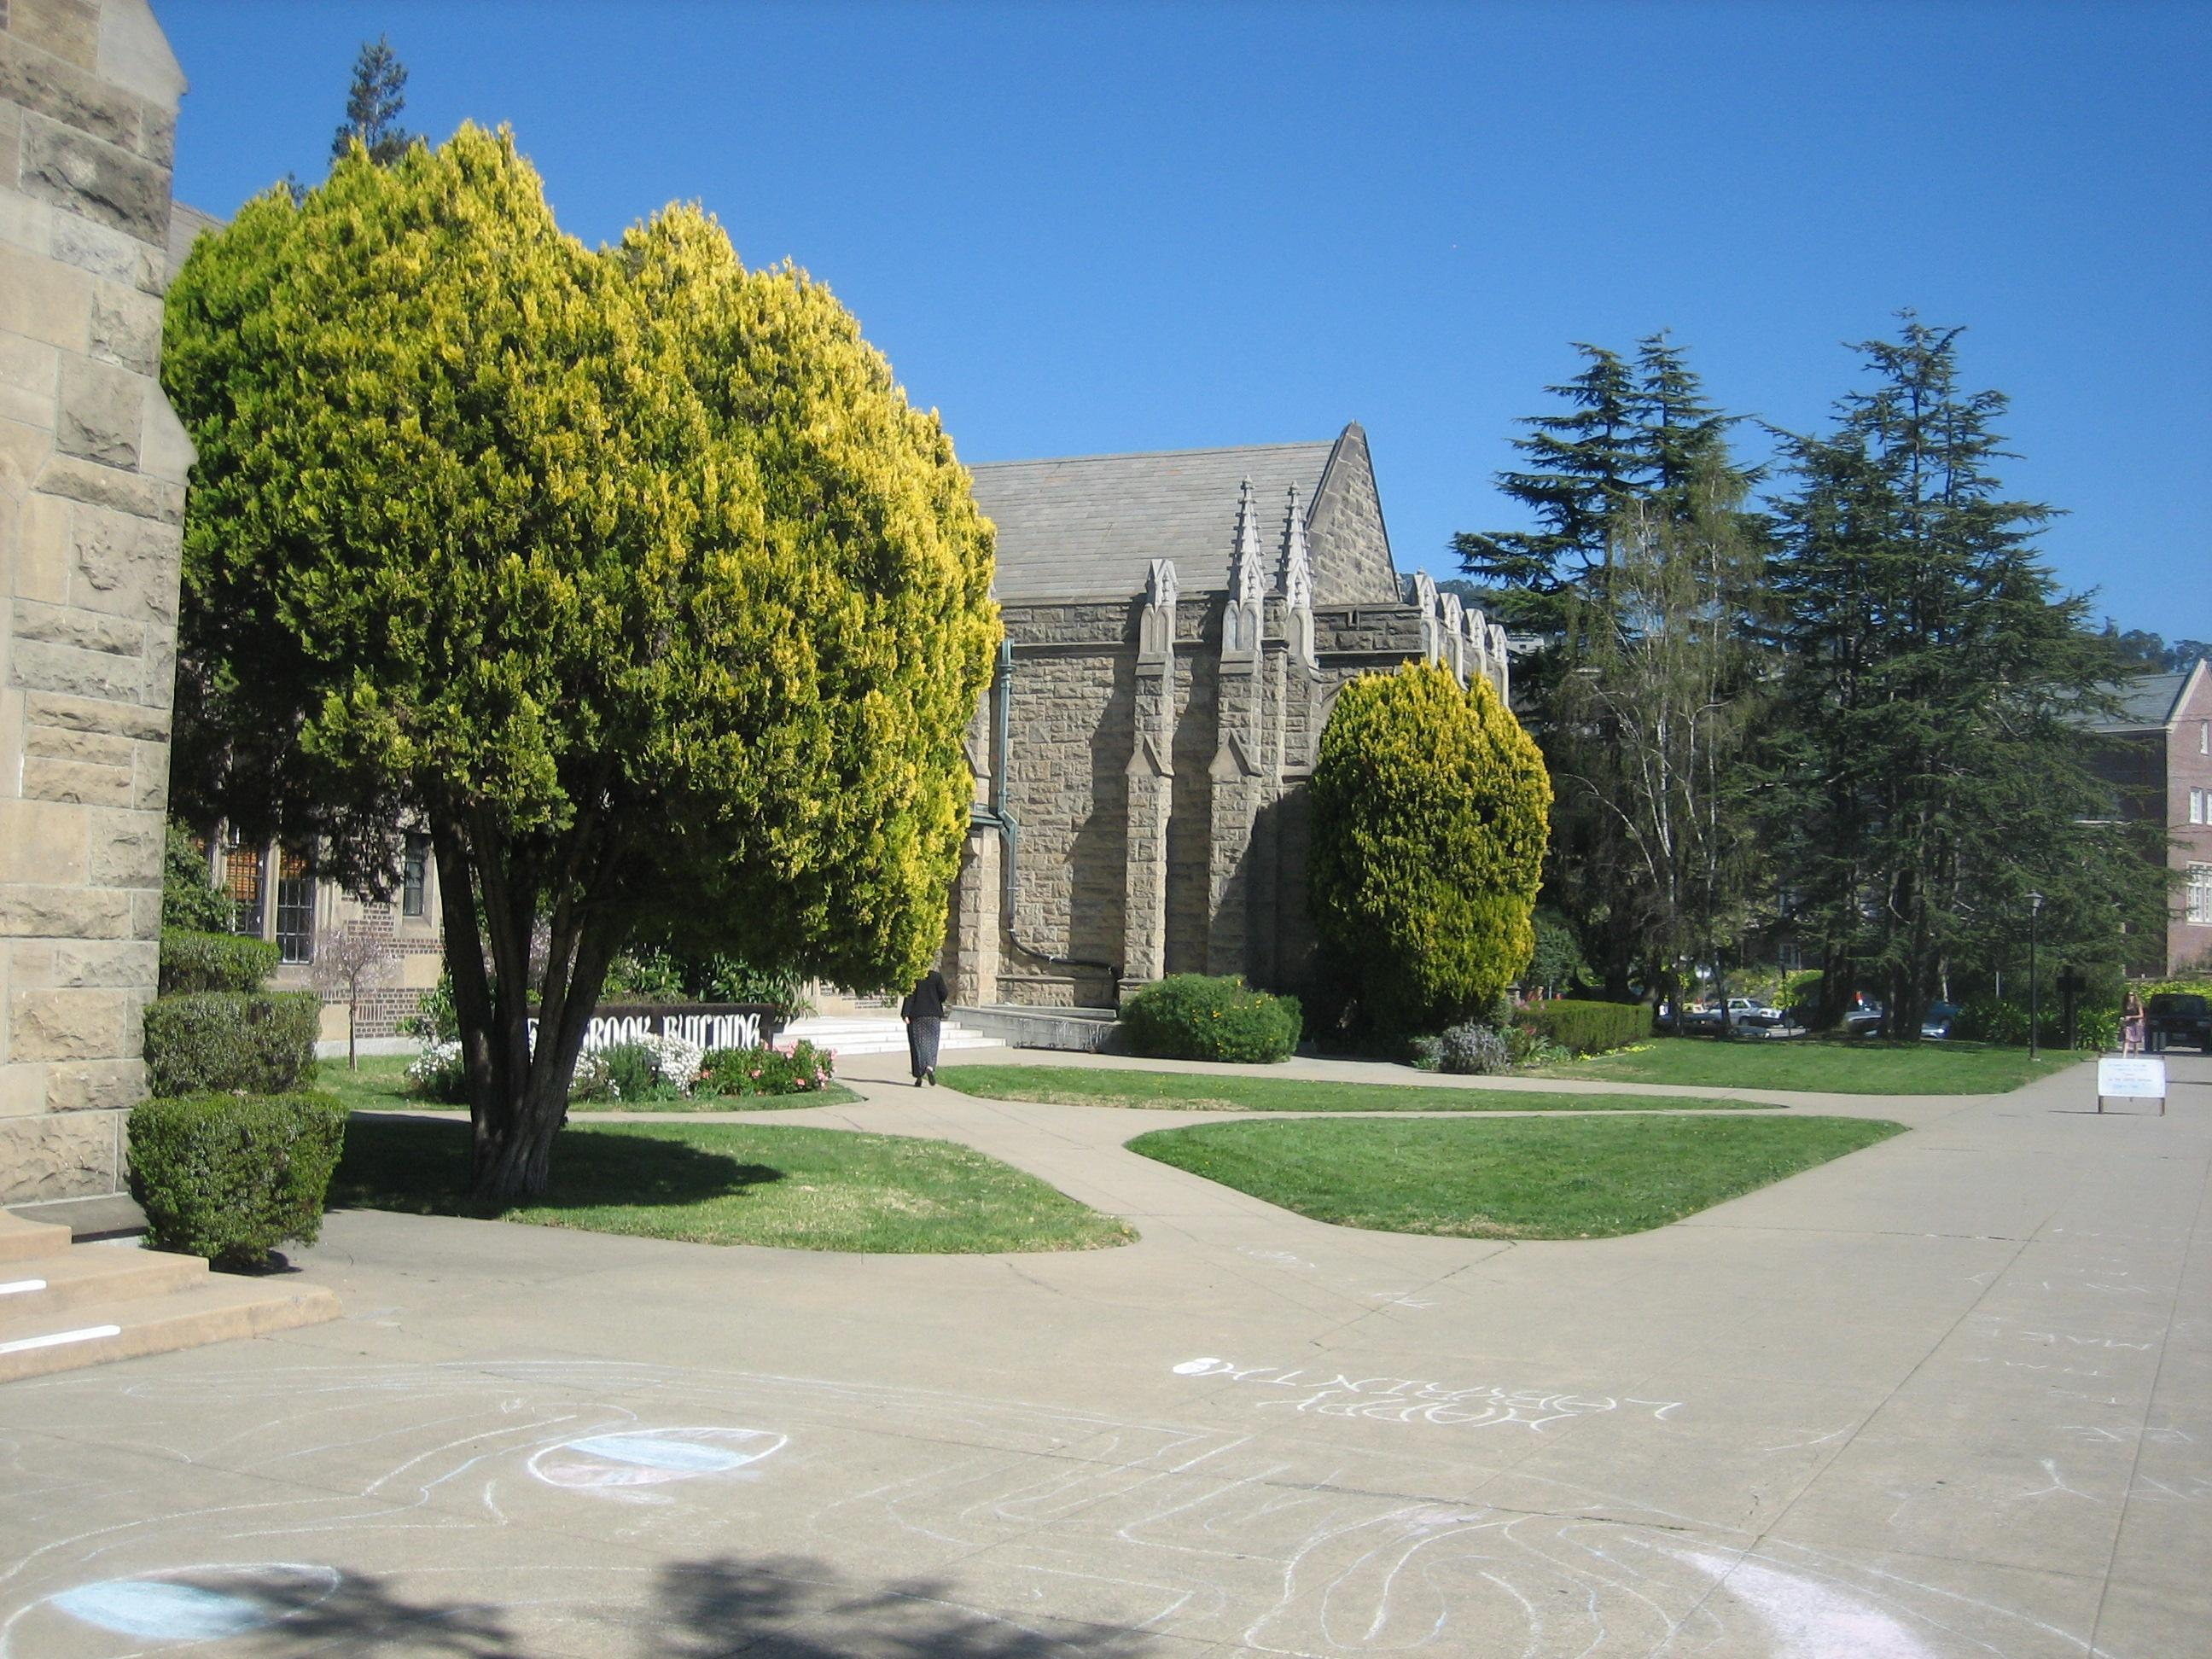
\includegraphics[width=2cm ,height=2cm ]{\input_image}};		
%	\draw [connection] (fake_image-north) -- node[fillwhite] {\midarrow} (semantic_map_2-nearsouth);
%	\path (semantic_map_2-west) -| node[fillwhite, align=center] (sem_loss) {\LARGE \bf\textit{Semantic}\\ \LARGE \bf\textit{loss}} (generator_north_1);
%	\draw [connection] (image_0) --  node[fillwhite] {\midarrow} (sem_loss);				
%	\draw [connection] (semantic_map_2-west)  --(image_1) -- node[fillwhite] {\midarrow}(sem_loss);
%	\draw [connection, densely dashed] (sem_loss) -- node[near end, fillwhite] {\midarrow} (generator_north_1);
%
%
%%Cycle consistency Loss	
%	\draw [connection] (fake_image-northwest) -- node [inner sep=0, fillwhite] (rec) {\midarrow} (generator-northeast);
%	\draw [connection] (attributes-east) -| node [pos=0.3, fillwhite] {\midarrow} (rec);
%	
%
%	\pic[shift={(-8, 0, -4)}] at (generator-farnorth)
%	{SolidBox={
%			name=rec_image,
%			fill=white,
%			height=10,
%			depth=10,
%			width={1}
%		}
%	};
%	\draw [connection] (generator-farnorth) -- node [fillwhite] {\midarrow} ++(0,0,-4) -| node [fillwhite] {} (rec_image-west);
%	\path (real_image-far) -- node [align=center] (cycle_loss) {\LARGE \bf\textit{Cycle}\\\LARGE \bf\textit{loss}} ++(0.5,0,-4.9);
%	\draw [connection, dashed] (cycle_loss) -- node [fillwhite] {\midarrow} (generator-northwest);
%	\draw [connection] (real_image-far) -- node [fillwhite, at end] {\midarrow} (cycle_loss.south west);
%	\draw [connection] (rec_image-near) -- node [fillwhite] {\midarrow} (cycle_loss);
%	\node [align=right, below left, inner sep=15] () at (rec_image-northwest) {\LARGE \bf Reconstructed \\ \LARGE \bf image};
%	
%% Discriminator
%	\pic[shift={(5, 1, 0)}] at (fake_image-north)	
%	{SolidBox={
%			name=discriminator,
%			label=\LARGE \bf Discriminator,
%			fill=red,
%			height=15,
%			depth=15,
%			width={20},
%			opacity=0.1
%		}
%	};	
%
%	\node (dummy) [shift={(-2.5,0,0)}, inner sep=15] at (discriminator-west) {};
%
%	\draw [connection] (fake_image-east) -| (dummy);
%	
%	\draw [connection] (real_images_2-east) -| (dummy) -- node [fillwhite] {\midarrow} (discriminator-west);
%	
%	\draw [connection] (dummy.south) -- (dummy.east);
%	\draw[ultra thick, draw=\edgecolor, <->, >=latex', shorten >= 3pt, shorten <= 3pt] (dummy.south) to [bend left](dummy.north);
%	\node[fill=\edgecolor, inner sep=2, circle] at (dummy.south) {};  
%	\node[fill=\edgecolor, fill, inner sep=2, circle] at (dummy.north) {};  
%	\node[fill=\edgecolor, fill, inner sep=2, circle] at (dummy.east) {};  
%	
%	
%	\node (real) [shift={(2,0.5,0)}, inner sep=0] at (discriminator-east) {\LARGE \bf Real};
%	\node (fake) [shift={(2,-0.5,0)}, inner sep=0] at (discriminator-east) {\LARGE \bf Fake};
%	\draw [connection] (discriminator-east) ++(0,0.5) -- ++(1,0) |- (real);
%	\draw [connection] (discriminator-east) ++(0,-0.5) -- ++(1,0) |- (fake);
%	\node [draw, diamond, thick, shift={(5,0,0)}, inner sep=1] (correct) at (discriminator-east) {\LARGE \bf Correct?};
%	\draw [connection] (correct.west) -- ++(-0.25,0)  node [coordinate] (dummy_2) {} |- (real.east) ;
%	\draw [connection] (fake) -| (dummy_2);
%	
%	\draw [connection, dashed] (correct) -- ++(2,0) -- node [fillwhite, rotate=90, near start, inner sep=2] {\LARGE \bf no} ++(0,-1) -- node [fillwhite] {\midarrow} ++(0,-4)  |- node [fill=white, opacity=1, near end, rotate=180] {\LARGE \bf\textit{Discriminator loss}} ++(-9,0) -| node [near end, fillwhite] {\midarrow} (discriminator-nearsouth);
%	
%	\draw [connection, dashed] (correct) ++(2,0) -- ++(1,0) -- node [fillwhite, rotate=90, pos=0.3, inner sep=2] {\LARGE \bf yes} ++(0,-1) -- node [fillwhite] {\midarrow} ++(0,-8) |- node [fill=white, opacity=1, rotate=180, near end] {\LARGE \bf\textit{Generator loss}} ++(-20,0) -| node [near end, fillwhite] {\midarrow} (generator_south_1);
%
%  	\node [fillwhite, align=center, inner sep=2] (test2) [below] at (fake_image-nearsouth) {\LARGE \bf Generated image};
	\end{tikzpicture}
\end{document}